\documentclass[a4paper,12pt]{article}
\usepackage{xcolor}
\usepackage{amsmath,amsfonts,amssymb}
\usepackage{geometry}
\usepackage{fancyhdr}
\usepackage{graphicx}
\usepackage{titlesec}
\usepackage{tikz}
\usepackage{booktabs}
\usepackage{array}
\usetikzlibrary{shadows}
\usepackage{tcolorbox}
\usepackage{float}
\usepackage{lipsum}
\usepackage{mdframed}
\usepackage{pagecolor}
\usepackage{mathpazo}   
\usepackage{microtype}  

\setlength{\parindent}{0pt}

% Page background color
\pagecolor{gray!10!white}

% Geometry settings
\geometry{margin=0.5in}
\pagestyle{fancy}
\fancyhf{}

% Fancy header and footer
\fancyhead[C]{\textbf{\color{blue!80}CS765 Project Part-1}}
% \fancyhead[R]{\color{blue!80}Saksham Rathi}
\fancyfoot[C]{\thepage}

% Custom Section Color and Format with Sans-serif font
\titleformat{\section}
{\sffamily\color{purple!90!black}\normalfont\Large\bfseries}
{\thesection}{1em}{}

% Custom subsection format
\titleformat{\subsection}
{\sffamily\color{cyan!80!black}\normalfont\large\bfseries}
{\thesubsection}{1em}{}

% Stylish Title with TikZ (Enhanced with gradient)
\newcommand{\cooltitle}[1]{%
\begin{tikzpicture}
\node[fill=blue!20,rounded corners=10pt,inner sep=12pt, drop shadow, top color=blue!50, bottom color=blue!30] (box)
{\Huge \bfseries \color{black} #1};
\end{tikzpicture}
}
\usepackage{float} % Add this package

\newenvironment{solution}[2][]{%
\begin{mdframed}[linecolor=blue!80, linewidth=2pt, roundcorner=10pt, backgroundcolor=yellow!10!white, skipabove=12pt, skipbelow=12pt]%
	\textbf{\large #2}
	\par\noindent\rule{\textwidth}{0.4pt}
}{
\end{mdframed}
}


\title{\cooltitle{CS765 Project Part-1} \\
\LARGE \textbf{Simulation of a P2P Cryptocurrency Network} \\
Design Document}
\author{{\bf Saksham Rathi (22B1003), Kavya Gupta (22B1053), Mayank Kumar (22B0933)} \\
\small Department of Computer Science, \\
Indian Institute of Technology Bombay \\}
\date{}

\begin{document}
\maketitle

% \newpage
% \begin{solution}{Introduction}
% 	This document provides the design details for the discrete-event simulator of a P2P cryptocurrency network. It describes the modular flow, event-driven structure, and code implementation details.
% \end{solution}

\newpage
\section*{Flowchart of Event Execution}
\begin{figure}[h]
    \centering
    \fbox{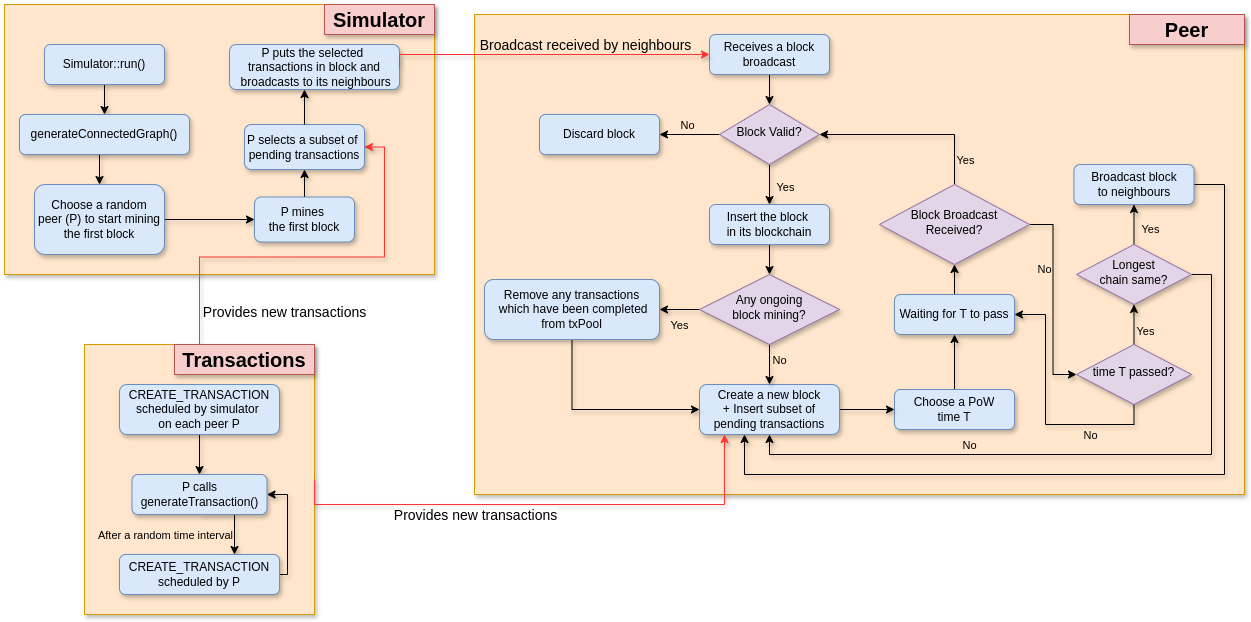
\includegraphics[width=1\textwidth]{../images/flowchart.png}}
    \caption{Flow of events}
\end{figure}

\subsection*{Simulator}

%%%%%%%%%%%%%%%%%%%%%%%%%%%%%%%%%%%%%%%%%%%%%%%%%%%%%%%%%%%%%%%%%%%%%%%%%%%%%%%%%%%%%%%%%%%%%%%%%%%%%%%%%%%%%%%%%%%%%%%%%%%%%%%%%%%%%%%%%%%%%%%%%%%%%%%%%%%%%%%%%%%%%%%%%%%%
\begin{itemize}
	\item The simulator calls the \texttt{run} function to start the simulation.
	\item It first calls the \texttt{generateConnectedGraph} function to create a connected graph of nodes.
	\item Each node then creates a genesis block using the \texttt{createGenesisBlock} function.
	\item The simulator schedules the creation of transactions by calling \texttt{scheduleEvent} with an inter-arrival time, event type, and node index.
\end{itemize}

% \begin{mdframed}[linecolor=black, linewidth=2pt, roundcorner=10pt, backgroundcolor=yellow!10!white, skipabove=12pt, skipbelow=12pt]
% \begin{verbatim}
% void Simulator::run() {
% 	generateConnectedGraph();
	
% 	for (int i = 0 ; i < num_nodes ; i++ ) {
% 		peers[i]->createGenesisBlock();
% 	}
	
% 	for (int i = 0 ; i < num_nodes ; i ++ ) {
% 		double interArrivalTime = getInterArrivalTime();
% 		scheduleEvent(interArrivalTime, CREATE_TRANSACTION, i, -1, {});
% 	}
% }
% \end{verbatim}
% \end{mdframed}
%%%%%%%%%%%%%%%%%%%%%%%%%%%%%%%%%%%%%%%%%%%%%%%%%%%%%%%%%%%%%%%%%%%%%%%%%%%%%%%%%%%%%%%%%%%%%%%%%%%%%%%%%%%%%%%%%%%%%%%%%%%%%%%%%%%%%%%%%%%%%%%%%%%%%%%%%%%%%%%%%%%%%%%%%%%%

%%%%%%%%%%%%%%%%%%%%%%%%%%%%%%%%%%%%%%%%%%%%%%%%%%%%%%%%%%%%%%%%%%%%%%%%%%%%%%%%%%%%%%%%%%%%%%%%%%%%%%%%%%%%%%%%%%%%%%%%%%%%%%%%%%%%%%%%%%%%%%%%%%%%%%%%%%%%%%%%%%%%%%%%%%%%
\begin{itemize}
	\item A random peer is selected to start mining by scheduling a \texttt{MINING\_START} event.
	\item The simulator processes events from the event queue by updating the current time and handling each event accordingly.
\end{itemize}

% \begin{mdframed}[linecolor=black, linewidth=2pt, roundcorner=10pt, backgroundcolor=yellow!10!white, skipabove=12pt, skipbelow=12pt]
% \begin{verbatim}
% 	int random_peer = uniformRandom(0, num_nodes - 1);
% 	scheduleEvent(currentTime, MINING_START, random_peer, -1, {});
% 	while ( !eventQueue.empty() ) {
% 		Event current = eventQueue.top();
% 		eventQueue.pop();
% 		currentTime = current.time;
% 		handleEvent(current);
% 	}
% \end{verbatim}
% \end{mdframed}
%%%%%%%%%%%%%%%%%%%%%%%%%%%%%%%%%%%%%%%%%%%%%%%%%%%%%%%%%%%%%%%%%%%%%%%%%%%%%%%%%%%%%%%%%%%%%%%%%%%%%%%%%%%%%%%%%%%%%%%%%%%%%%%%%%%%%%%%%%%%%%%%%%%%%%%%%%%%%%%%%%%%%%%%%%%%

\subsection*{Transactions}
%%%%%%%%%%%%%%%%%%%%%%%%%%%%%%%%%%%%%%%%%%%%%%%%%%%%%%%%%%%%%%%%%%%%%%%%%%%%%%%%%%%%%%%%%%%%%%%%%%%%%%%%%%%%%%%%%%%%%%%%%%%%%%%%%%%%%%%%%%%%%%%%%%%%%%%%%%%%%%%%%%%%%%%%%%%%
A peer creates a transaction by calling the \texttt{generateTransaction} function.
	\begin{itemize}
		\item The peer checks its balance using the \texttt{getPeerBalance} function.
		\item If the balance is greater than zero, it selects a random target peer.
		\item A transaction is created and added to the transaction pool.
		\item The transaction is then broadcasted to all neighboring peers.
	\end{itemize}

% \begin{mdframed}[linecolor=black, linewidth=2pt, roundcorner=10pt, backgroundcolor=yellow!10!white, skipabove=12pt, skipbelow=12pt]
% 	\begin{verbatim}
% 		void Peer::generateTransaction() {
% 			double our_balance = blockchain->getPeerBalance(id);
% 			if (our_balance <= 0) {
% 				return;
% 			}
			
% 			int targetPeerID = id;
% 			while (targetPeerID == id) {
% 				targetPeerID = uniformRandom(0, num_nodes - 1);
% 			}
% 			Transaction txn = Transaction(id, targetPeerID,uniformRandom(1, our_balance));
% 			txPool.insert(txn);
% 			for (auto& [id, peer] : neighbours) {
% 				sendTransaction(txn, peer->id);
% 			}
% 		}
% 	\end{verbatim}
% \end{mdframed}
%%%%%%%%%%%%%%%%%%%%%%%%%%%%%%%%%%%%%%%%%%%%%%%%%%%%%%%%%%%%%%%%%%%%%%%%%%%%%%%%%%%%%%%%%%%%%%%%%%%%%%%%%%%%%%%%%%%%%%%%%%%%%%%%%%%%%%%%%%%%%%%%%%%%%%%%%%%%%%%%%%%%%%%%%%%%

\newpage
%%%%%%%%%%%%%%%%%%%%%%%%%%%%%%%%%%%%%%%%%%%%%%%%%%%%%%%%%%%%%%%%%%%%%%%%%%%%%%%%%%%%%%%%%%%%%%%%%%%%%%%%%%%%%%%%%%%%%%%%%%%%%%%%%%%%%%%%%%%%%%%%%%%%%%%%%%%%%%%%%%%%%%%%%%%%
After the simulator first schedules the event \texttt{CREATE\_TRANSACTION} at each node:
    \begin{itemize}
        \item Each node generates a transaction and then a new time (\texttt{newTime}) is calculated by adding the current time to a value obtained from an exponential distribution using the function \texttt{getInterArrivalTime()}.
        \item The event \texttt{CREATE\_TRANSACTION} is then recursively scheduled on the same node with the newly calculated \texttt{newTime}.
    \end{itemize}

% \begin{mdframed}[linecolor=black, linewidth=2pt, roundcorner=10pt, backgroundcolor=yellow!10!white, skipabove=12pt, skipbelow=12pt]
% \begin{verbatim}
% case CREATE_TRANSACTION:
% 	peers[event.sourcePeer]->generateTransaction();
% 	newTime = currentTime + getInterArrivalTime();
% 	scheduleEvent(newTime, CREATE_TRANSACTION, event.sourcePeer, -1, event.data);
% 	break;
% 	\end{verbatim}
% \end{mdframed}
%%%%%%%%%%%%%%%%%%%%%%%%%%%%%%%%%%%%%%%%%%%%%%%%%%%%%%%%%%%%%%%%%%%%%%%%%%%%%%%%%%%%%%%%%%%%%%%%%%%%%%%%%%%%%%%%%%%%%%%%%%%%%%%%%%%%%%%%%%%%%%%%%%%%%%%%%%%%%%%%%%%%%%%%%%%%

\section*{Peer}

\subsection*{Receiving the Blocks}
\begin{itemize}
	\item The peer first checks if the block has not been seen before. If the block has not been seen, it stores the block's timestamp.
	\item Then, it checks if the parent of the received block is present in its blockchain. If the parent is not present, the block ID of the block is stored in a set.
	\item This block without a parent will be checked later when its parent arrives.
\end{itemize}

\subsection*{Validating the Received Block}

\begin{itemize}
    \item The peer validates the block by checking if the parent block exists in the blockchain.
    \item It initializes the balance of each peer to the initial balance and then iterates through the current block and its parent blocks, updating the balances based on the transactions.
    \item For each transaction, the sender's balance is decreased, and the receiver's balance is increased by the transaction amount.
    \item The miner of each block receives a mining reward added to their balance.
    \item If any peer's balance becomes negative during this process, the block is considered invalid.
\end{itemize}

\subsection*{Inserting the Block in the Blockchain}

\begin{itemize}
    \item Given the block is valid, it is inserted into the blockchain of the peer.
    \item The process of identifying the longest chain in the tree is then done and respective fields updated accordingly.
    \item Finally, it is checked if any children of the current block had arrived early on the peer. If so, then it is also inserted into the tree if it is still valid.
\end{itemize}

After all these steps, the information of the block is sent to the neighbors of the block. In case of the child blocks arriving before the parent blocks, 
their information is withheld with the peer till their parent arrives. 
\textit{This ensures that the blockchain remains consistent and valid.}

\subsection*{Mining a Block}

\begin{itemize}
    \item \textbf{MINING\_START:} In this event, the peer selects a subset of pending transactions from the transaction pool (txPool) and creates a block. The peer ensures that the sender has sufficient balance for each transaction before adding it to the block. The block is then prepared with the necessary details such as parent ID, miner ID, and height.
    \item \textbf{MINING\_END:} This event is scheduled and added to the event queue after MINING\_START. During this event, it is first checked if the longest chain is the same as when the MINING\_START was scheduled. If the chain is unchanged, the block is inserted into the blockchain and sent to the peer's neighbors. If the chain has changed, the block is discarded and the mining process is started again.
\end{itemize}

\section*{Helper Functions}

\subsection*{generateConnectedGraph}

\begin{itemize}
    \item \textbf{Initialize Peer IDs:} The function starts by creating a list of peer IDs from the peers array. The peer IDs are shuffled to ensure randomness in the graph structure.
    \item \textbf{Create Initial Chain:} The function creates a chain of connections between peers to ensure the graph is connected. This is done by iterating through the shuffled peer IDs and connecting each peer to the next one in the list.
    \item \textbf{Ensure Minimum Degree:} To ensure that each peer has at least 3 connections, the function adds edges between the current peer and a randomly selected peer, ensuring that the randomly selected peer has fewer than 6 connections and is not already connected to the current peer.
\end{itemize}

\subsection*{handleEvent}

\begin{itemize}
    \item \textbf{Event Handling:} The function processes different types of events such as mining start, mining end, transaction creation, transaction sending, transaction receiving, block sending, and block receiving. Each event type triggers specific actions performed by the peers.
    \item \textbf{Event Scheduling:} When an event is processed, the function calculates the time for the next event based on the current time and specific conditions such as block inter-arrival time, transaction inter-arrival time, or network latency.
    \item \textbf{Event Queue:} The calculated future event is then scheduled by adding it to an event queue. This queue ensures that events are processed in the correct order based on their scheduled times.
    \item \textbf{Simulation Flow:} The event queue drives the simulation flow by continuously processing and scheduling events, allowing the simulation to progress through different states and interactions between peers.
\end{itemize}

\section*{Additional Features}

\subsection*{Handling of Blocks with Invalid Parent ID}

\begin{itemize}
    \item If the parent of the received block is not present in the blockchain, the block ID is stored in a set.
    \item Blocks without a parent will be checked later when their parent arrives.
    \item If any children of the current block had arrived earlier, they are also inserted into the blockchain if they are still valid.
    \item After these steps, the block information is sent to the neighboring peers.
    \item In case child blocks arrive before their parent blocks, their information is withheld until the parent block arrives.
\end{itemize}

\end{document}
